\documentclass[11pt]{article}
\usepackage[margin=1in]{geometry}
\usepackage{amsmath,amssymb,booktabs,graphicx,url}
\usepackage{microtype}
\title{APG-AMS: Entropy-Guided Screening for Adaptive Metric Search in Distance-Based Learning}
\author{Mohammad Amir Khusru Akhtar\\Usha Martin University, Ranchi--834001, Jharkhand, India\\\texttt{akakhtar.2024@gmail.com}}
\date{}
\begin{document}
\maketitle

\begin{abstract}
Distance-based learning algorithms depend critically on the choice of metric, while exhaustive local search over candidate Minkowski norms increases computational cost through repeated distance evaluations. We present Arithmetic Power Geometry Adaptive Metric Selection (APG-AMS), an entropy-guided screening framework that uses normalized entropy of squared-coordinate weights to identify queries for which adaptive metric search may be unnecessary. The method is motivated by a local APG exponent-deformation result near the Euclidean reference exponent $p=2$, where first-order sensitivity of normalized power-sum distortion is governed by Shannon entropy. We expanded the empirical evaluation to 12 benchmark, controlled, and real-world datasets and compared APG-AMS with Euclidean $k$-nearest neighbors, full adaptive $p$-search, Neighborhood Components Analysis (NCA), and Large Margin Nearest Neighbor (LMNN) under common 10-fold stratified folds. Across 120 matched dataset-fold units, mean accuracy was 0.9267 for APG-AMS, 0.9260 for Euclidean $k$-NN, 0.9309 for full $p$-search, 0.9443 for NCA, and 0.9334 for LMNN. APG-AMS was statistically indistinguishable from Euclidean $k$-NN in accuracy (paired $t$-test $p=0.326$; Wilcoxon $p=0.512$), while the 0.42-percentage-point mean deficit relative to full $p$-search was statistically detectable. APG-AMS reduced candidate metric-search evaluations by 66.47\% on average across the 12 dataset summaries. These results support APG-AMS as a computational screening layer that trades a small amount of predictive performance relative to exhaustive or learned metric adaptation for reduced adaptive-search effort; it is not proposed as a replacement for supervised metric learning.
\end{abstract}

\noindent\textbf{Keywords:} Arithmetic Power Geometry; adaptive metric selection; $k$-nearest neighbors; Shannon entropy; metric learning; Minkowski distance.

\section{Introduction}
Distance is a central computational primitive in machine learning. Nearest-neighbor classification, clustering, manifold learning, retrieval, and similarity search depend on the geometry induced by the chosen metric \cite{cover1967,bishop2006,hastie2009,murphy2012}. The classical $k$-nearest-neighbor ($k$-NN) rule is simple and interpretable, but its performance can vary substantially with the distance function \cite{cover1967,devroye1996,cunningham2021}. Metric learning therefore remains an important research topic \cite{xing2003,goldberger2005,weinberger2009,kulis2013,bellet2013}.

A common alternative to learning a full transformation is to search over candidate Minkowski norms. Full local search can adapt neighborhood geometry, but it repeats distance calculations for every candidate metric. The practical question motivating this work is therefore not only which metric should be used, but also when adaptation is unnecessary.

Arithmetic Power Geometry (APG) treats the norm exponent as a deformation parameter around the Euclidean reference state $p=2$. In the local APG setting, first-order sensitivity under exponent deformation is governed by the Shannon entropy of squared-coordinate weights. This observation motivates APG-AMS: low-entropy queries are screened as metric-stable and evaluated with $L_2$, while high-entropy queries trigger a full local search over candidate $p$ values.

The revised paper makes five contributions. First, it states and proves a $d$-dimensional APG local sensitivity theorem for normalized power-sum distortion. Second, it formulates APG-AMS as a reproducible entropy-guided screening algorithm. Third, it evaluates the framework on 12 datasets spanning standard benchmarks, controlled stress tests, and four additional real-world UCI datasets. Fourth, it directly compares APG-AMS with Euclidean $k$-NN, exhaustive local $p$-search, NCA, and LMNN under common 10-fold stratified folds. Fifth, it reports paired tests over 120 matched dataset-fold units and provides an automated public reproducibility workflow. The contribution is a computation--accuracy trade-off rather than a claim of predictive superiority over supervised metric learning.

\section{Background and Related Work}
\subsection{Nearest-neighbor classification and metric dependence}
The $k$-NN rule is among the earliest nonparametric classifiers \cite{cover1967}. Its asymptotic behavior is well studied \cite{devroye1996}, but neighborhood quality remains metric-dependent.

\subsection{Metric learning}
Neighborhood Components Analysis (NCA) optimizes a stochastic nearest-neighbor objective \cite{goldberger2005}. Large Margin Nearest Neighbor (LMNN) learns a Mahalanobis transformation intended to keep target neighbors close while separating differently labeled samples \cite{weinberger2009}. These methods can improve prediction but require a supervised training stage \cite{kulis2013,bellet2013}. APG-AMS addresses a different decision: whether local search over candidate Minkowski exponents should be executed for a query. The revised experiments include NCA+$k$-NN and LMNN+$k$-NN as direct empirical baselines without claiming that they optimize the same objective.

\subsection{Entropy and information geometry}
For a probability vector $W=(w_1,\ldots,w_d)$, Shannon entropy is $H(W)=-\sum_i w_i\log w_i$ \cite{shannon1948,coverthomas2006}. Information geometry studies statistical models through geometric structures \cite{amari2016,nielsen2020}. APG-AMS uses entropy of squared feature-coordinate weights, not class entropy.

\section{Theory}
Let $x=(x_1,\ldots,x_d)\in\mathbb{R}_{>0}^d$ and define
\begin{equation}
S_2(x)=\sum_{i=1}^d x_i^2.
\end{equation}
For $p>0$, define the normalized power-sum ratio
\begin{equation}
R_p(x)=\frac{\sum_{i=1}^d x_i^p}{\left(\sum_{i=1}^d x_i^2\right)^{p/2}}.
\end{equation}
At $p=2$, $R_2(x)=1$. Let $K_P=p-2$ and define
\begin{equation}
w_i=\frac{x_i^2}{\sum_{j=1}^d x_j^2},\qquad \sum_i w_i=1,
\end{equation}
with
\begin{equation}
H(W)=-\sum_{i=1}^d w_i\log w_i,
\qquad
\bar H(W)=\frac{H(W)}{\log d}\quad(d>1).
\end{equation}

\paragraph{Theorem 1 (APG local entropy sensitivity).}
For fixed $x\in\mathbb{R}_{>0}^d$ and $p=2+K_P$ with $K_P\to0$,
\begin{equation}
R_p(x)=1-\frac{H(W)}{2}K_P+O(K_P^2).
\end{equation}
Consequently, for $\delta_K(x,p)=|1-R_p(x)|$,
\begin{equation}
\delta_K(x,p)=\frac{H(W)}{2}|K_P|+O(K_P^2).
\end{equation}

\paragraph{Proof.}
Using $x_i^{2+K_P}=x_i^2\exp(K_P\log x_i)$,
\begin{equation}
\sum_i x_i^{2+K_P}
=S_2(x)+K_P\sum_i x_i^2\log x_i+O(K_P^2).
\end{equation}
Also,
\begin{equation}
S_2(x)^{1+K_P/2}
=S_2(x)\left(1+\frac{K_P}{2}\log S_2(x)+O(K_P^2)\right).
\end{equation}
Hence
\begin{align}
R_{2+K_P}(x)
&=1+K_P\left[
\frac{\sum_i x_i^2\log x_i}{S_2(x)}
-\frac12\log S_2(x)\right]+O(K_P^2)\\
&=1+\frac{K_P}{2}\sum_i w_i\log w_i+O(K_P^2)\\
&=1-\frac{H(W)}{2}K_P+O(K_P^2).
\end{align}
Taking absolute deviation from one gives the result.

\paragraph{Scope clarification.}
Theorem 1 is local near $p=2$. It does not imply that APG entropy globally replaces exact Minkowski distances or learned metric methods, nor that the first-order expansion remains quantitatively accurate at large deviations such as $p=1$ or $p=4$. The adaptive search stage is empirical; the theorem motivates the screening variable.

\section{Methodology}
\subsection{APG-AMS}
For each test query $x$, APG-AMS computes $\bar H(W_x)$. With threshold $\tau$,
\begin{equation}
\mathrm{metric}(x)=
\begin{cases}
L_2, & \bar H(W_x)<\tau,\\
\arg\max_{p\in\{1,1.5,2,3,4\}}\mathrm{local\ purity}_k(x;p),
& \bar H(W_x)\ge\tau.
\end{cases}
\end{equation}
Local purity is the majority-class proportion among the $k$ nearest neighbors for a candidate $p$. We retain $k=7$, $\tau=0.92$, and $\mathcal P=\{1,1.5,2,3,4\}$ for comparability with the submitted manuscript. Full adaptive search evaluates all five candidates for every query; APG-AMS evaluates only $L_2$ for screened queries and all five candidates for entropy-sensitive queries.

\subsection{Datasets}
Twelve datasets were evaluated. The original suite contains Iris, Wine, Breast Cancer Wisconsin Diagnostic, Digits, Synthetic-20D, Synthetic-50D, Two Moons, and Concentric Circles. Four additional real-world UCI datasets were included in response to the reviews: Ionosphere (351 instances, 34 features), Sonar (208 instances, 60 features), Banknote Authentication (1,372 instances, 4 features), and Mice Protein Expression (1,080 instances, 77 usable feature columns in the implemented classification table). The added datasets broaden the evaluation across radar, sonar, image-derived, and biological measurements.

\subsection{Evaluation protocol}
All methods use identical outer 10-fold stratified splits. Missing-value imputation, when needed, is fit on the training fold only, followed by training-fold-only standardization. NCA and LMNN are fit exclusively on each standardized training fold and then applied to the corresponding test fold. Accuracy and weighted F1 are reported for all five methods. End-to-end fold runtime includes transformation learning for NCA/LMNN. Candidate-search reduction is reported separately for APG-AMS:
\begin{equation}
\mathrm{Reduction}=100\left(1-\frac{\mathrm{APG\ search\ units}}{\mathrm{full\ adaptive\ search\ units}}\right).
\end{equation}
Paired $t$-tests and Wilcoxon signed-rank tests are computed over the 120 matched dataset-fold units.

\section{Results}
\subsection{Expanded comparison}
Table~\ref{tab:main} reports mean 10-fold accuracy and APG search reduction. NCA and LMNN are included as established supervised metric-learning baselines.

\begin{table}[ht]
\centering
\caption{Mean 10-fold accuracy for the five methods; the final column reports APG-AMS candidate-search reduction.}
\label{tab:main}
\small
\begin{tabular}{lrrrrrr}
\toprule
Dataset & L2 & Full-$p$ & APG-AMS & NCA & LMNN & Red. (\%)\\
\midrule
Banknote & .9985 & .9985 & .9985 & 1.0000 & .9985 & 80.00\\
Breast Cancer & .9649 & .9666 & .9631 & .9736 & .9631 & 70.29\\
Concentric Circles & 1.0000 & 1.0000 & 1.0000 & 1.0000 & 1.0000 & 80.00\\
Digits & .9744 & .9777 & .9738 & .9777 & .9777 & 44.43\\
Ionosphere & .8375 & .8544 & .8432 & .8460 & .8517 & 58.11\\
Iris & .9600 & .9600 & .9600 & .9533 & .9600 & 80.00\\
Mice Protein & .9815 & .9861 & .9833 & .9889 & .9981 & 48.52\\
Sonar & .7981 & .8029 & .7933 & .8407 & .8026 & 67.64\\
Synthetic-20D & .8450 & .8600 & .8450 & .9160 & .8620 & 72.32\\
Synthetic-50D & .8120 & .8250 & .8200 & .8770 & .8480 & 37.28\\
Two Moons & .9730 & .9730 & .9730 & .9750 & .9720 & 80.00\\
Wine & .9667 & .9667 & .9667 & .9833 & .9667 & 79.11\\
\bottomrule
\end{tabular}
\end{table}

Across 120 matched dataset-fold units, mean accuracy was 0.92667 for APG-AMS, 0.92596 for Euclidean $k$-NN, 0.93091 for full adaptive $p$-search, 0.94431 for NCA, and 0.93338 for LMNN. Mean weighted F1 was 0.92484, 0.92402, 0.92934, 0.94290, and 0.93180, respectively.

\subsection{Paired statistical testing}
Table~\ref{tab:stats} summarizes paired accuracy comparisons.

\begin{table}[ht]
\centering
\caption{Paired accuracy comparisons over 120 matched dataset-fold units. Differences are APG-AMS minus comparator.}
\label{tab:stats}
\begin{tabular}{lrrr}
\toprule
Comparator & Mean difference & paired $t$ $p$ & Wilcoxon $p$\\
\midrule
L2 & +0.00071 & 0.325820 & 0.511781\\
Full-$p$ & -0.00425 & 0.000616 & 0.000752\\
NCA & -0.01764 & $4.35\times10^{-6}$ & $4.73\times10^{-7}$\\
LMNN & -0.00671 & $4.39\times10^{-5}$ & $4.13\times10^{-5}$\\
\bottomrule
\end{tabular}
\end{table}

APG-AMS remains statistically indistinguishable from Euclidean $k$-NN. The expanded study no longer supports the earlier claim of statistical indistinguishability from full adaptive $p$-search: the mean difference is only about 0.42 percentage points, but it is detectable over the enlarged paired sample. NCA and LMNN also achieve higher mean predictive accuracy than APG-AMS.

\subsection{Search reduction and real-world additions}
Across the 12 dataset summaries, mean APG-AMS candidate-search reduction is 66.47\%. On the four added real-world datasets, the accuracy/search-reduction pairs are 0.9985/80.00\% for Banknote Authentication, 0.8432/58.11\% for Ionosphere, 0.9833/48.52\% for Mice Protein Expression, and 0.7933/67.64\% for Sonar.

\begin{figure}[ht]
\centering
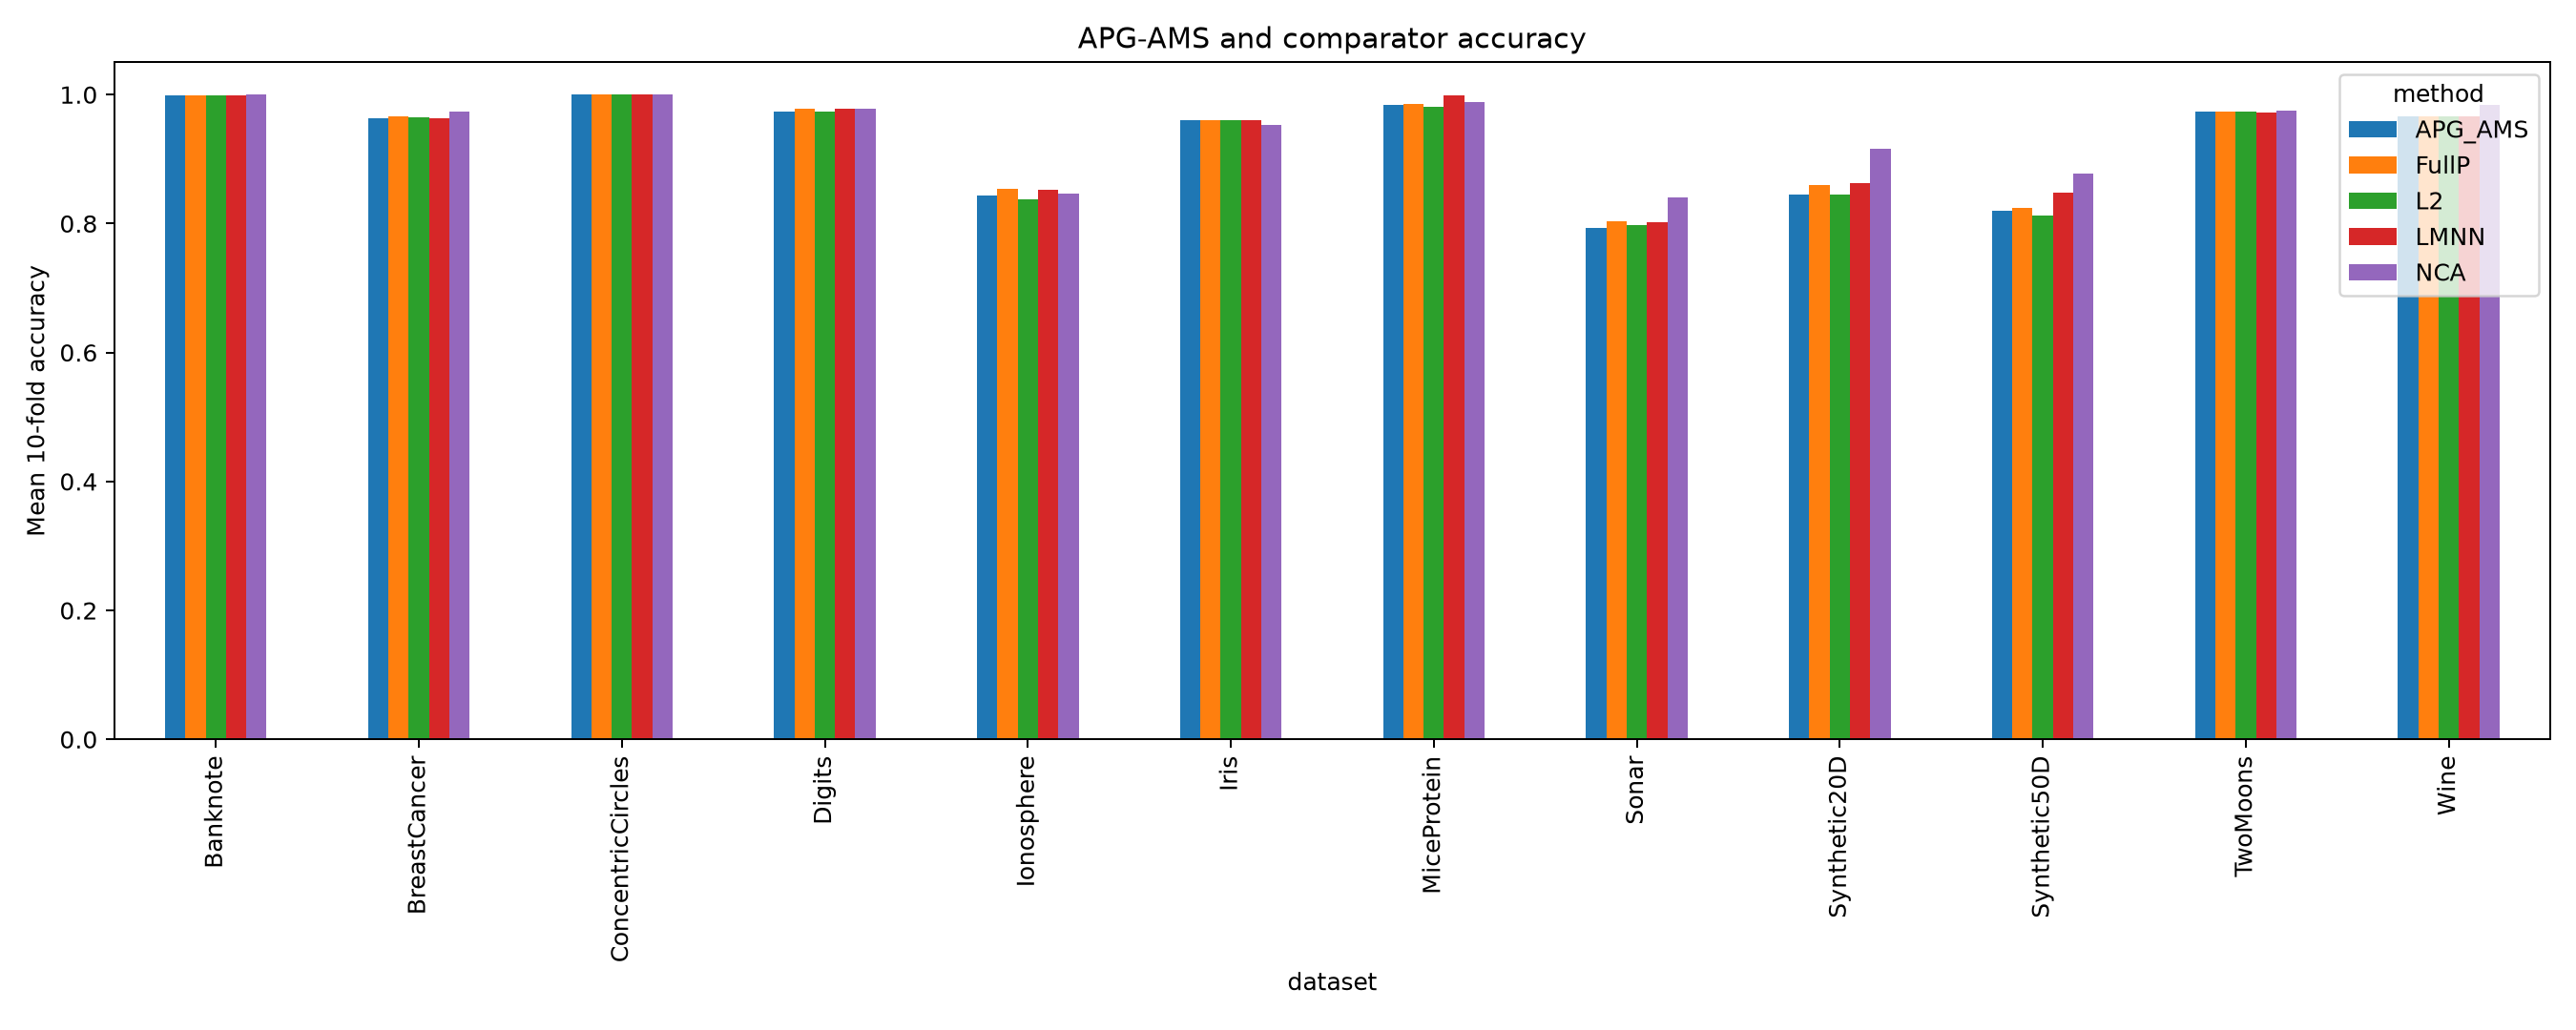
\includegraphics[width=.95\linewidth]{../results/accuracy_comparison.png}
\caption{Accuracy comparison generated by the reproducibility workflow.}
\label{fig:accuracy}
\end{figure}

\begin{figure}[ht]
\centering
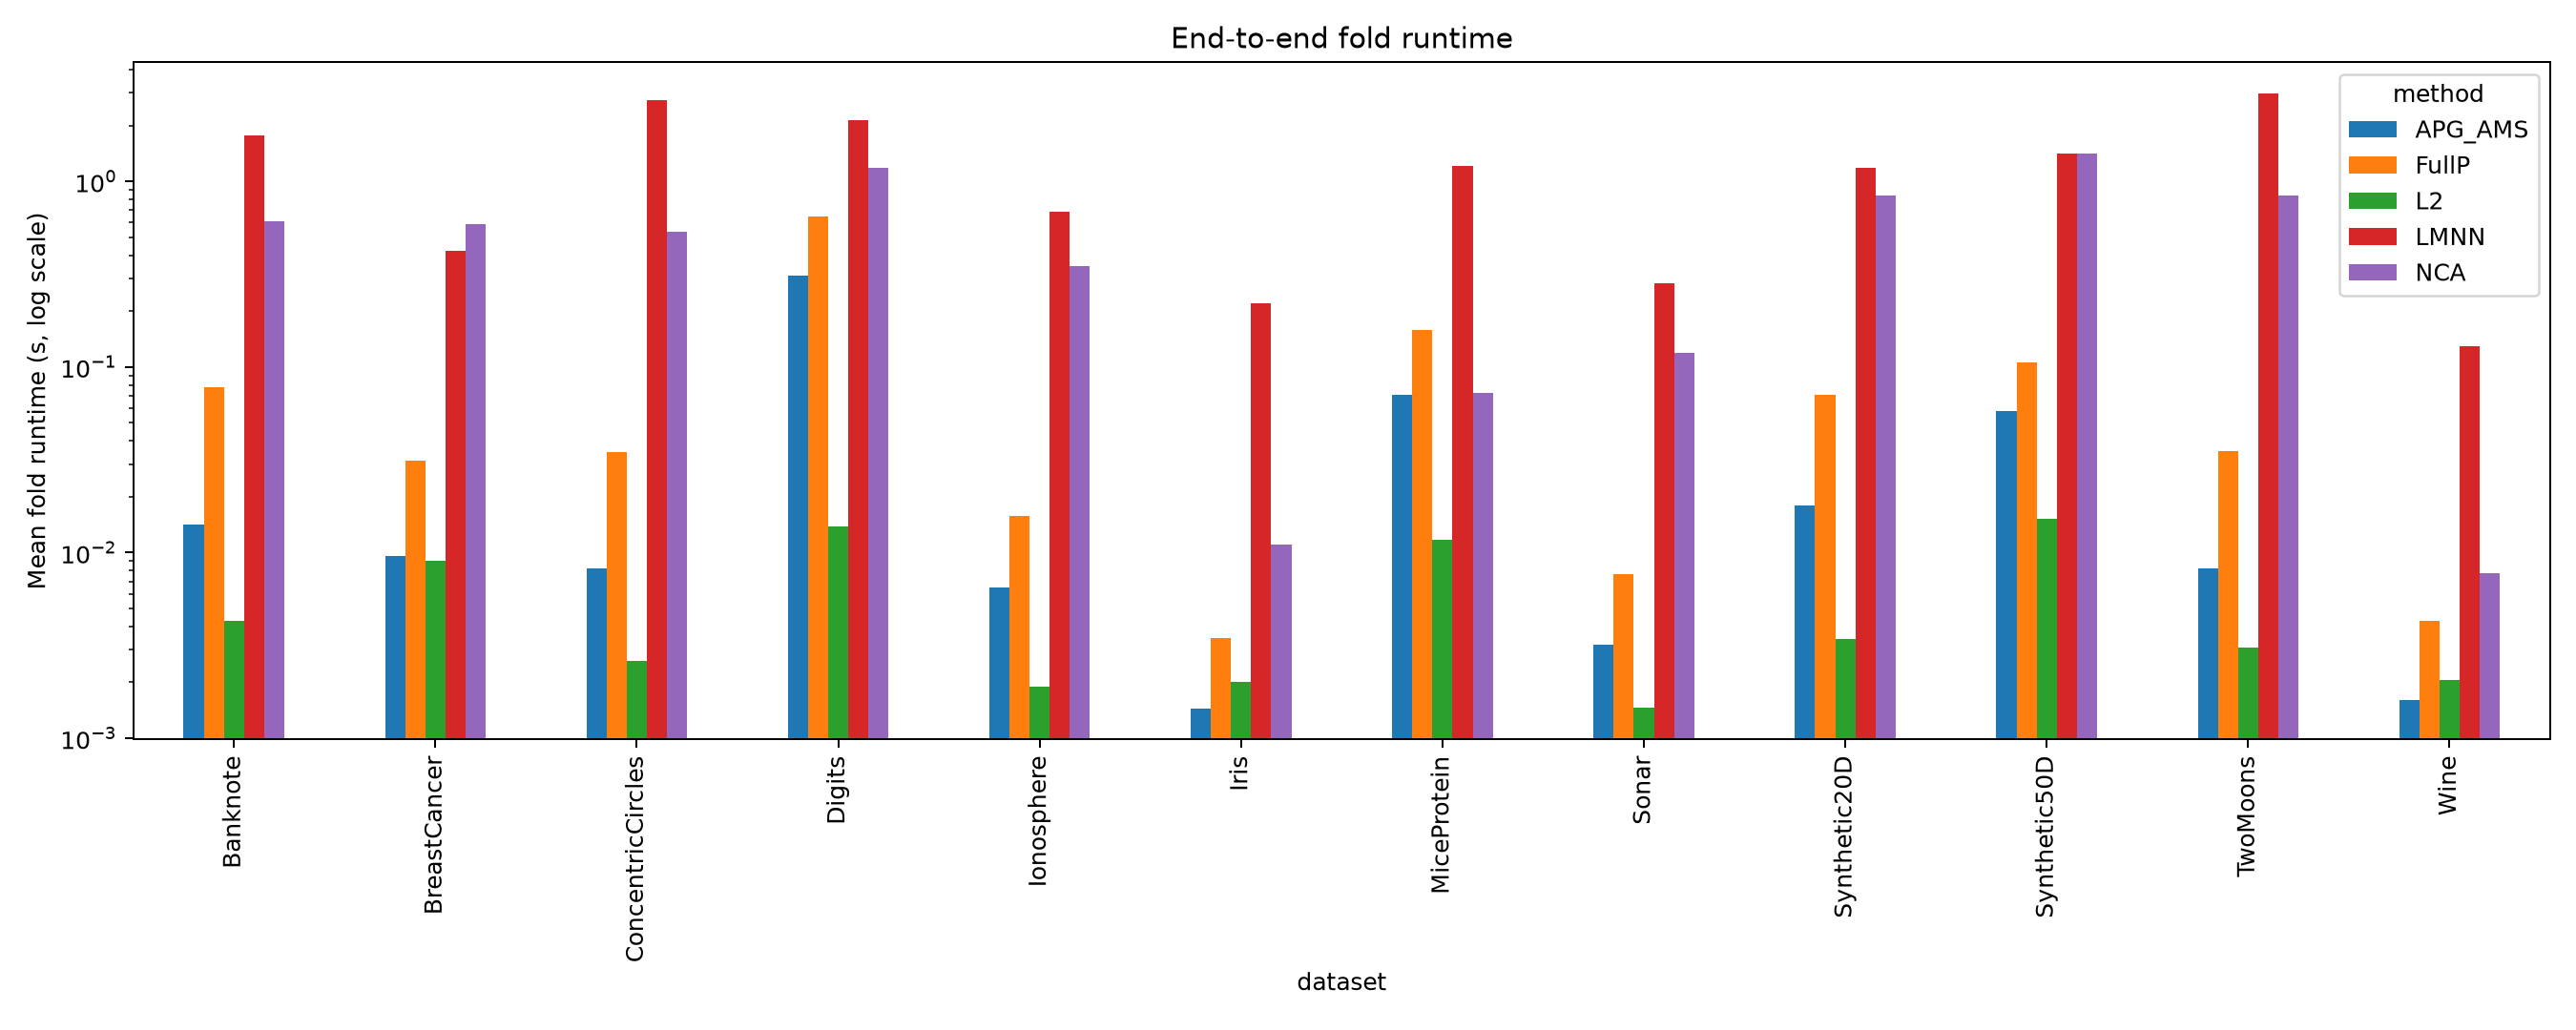
\includegraphics[width=.95\linewidth]{../results/runtime_comparison.png}
\caption{End-to-end fold runtime comparison on a logarithmic scale.}
\label{fig:runtime}
\end{figure}

\begin{figure}[ht]
\centering
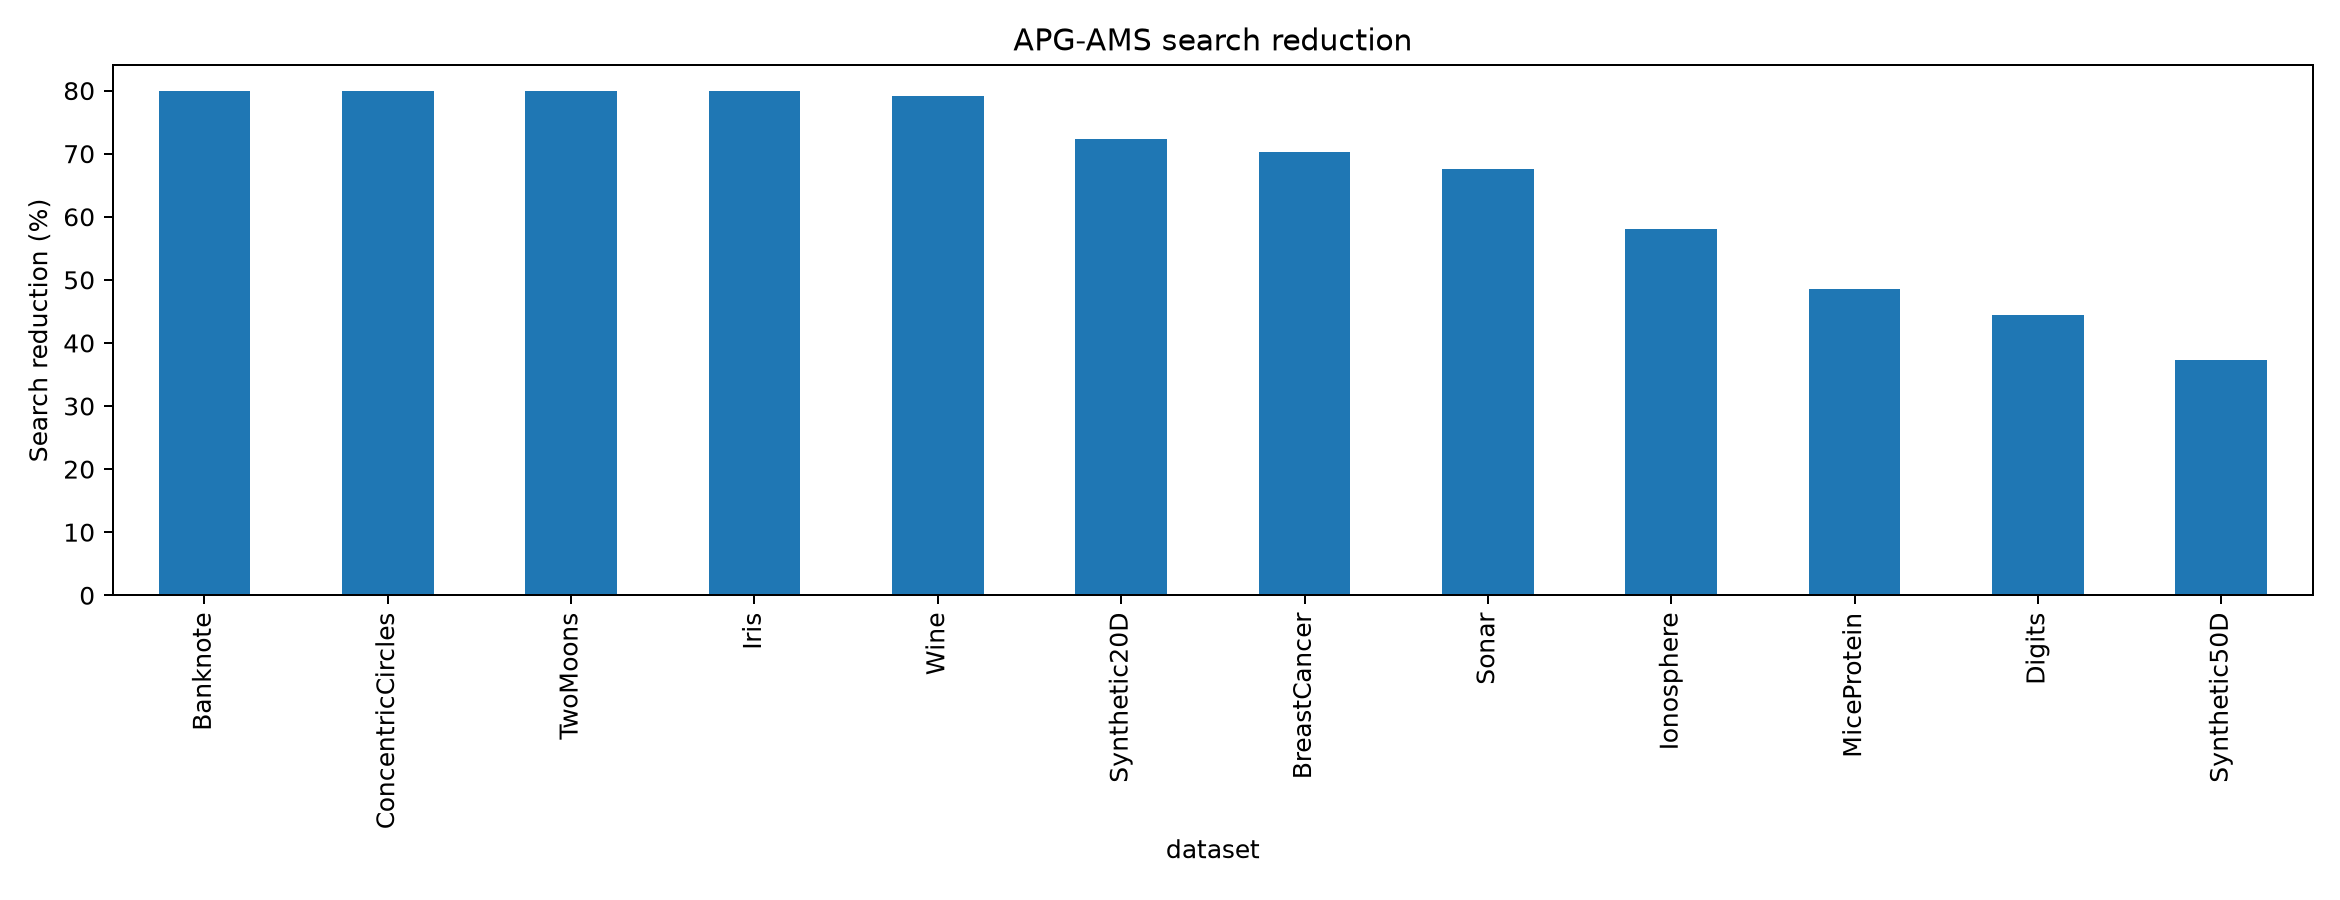
\includegraphics[width=.95\linewidth]{../results/search_reduction.png}
\caption{APG-AMS candidate-search reduction across datasets.}
\label{fig:reduction}
\end{figure}

\section{Discussion}
The expanded experiments refine the interpretation of APG-AMS. Its strongest result is not predictive dominance. APG-AMS achieves mean accuracy essentially equal to Euclidean $k$-NN while reducing candidate metric-search evaluations by 66.47\% on average. Full adaptive $p$-search gains approximately 0.42 percentage points in mean accuracy, and NCA and LMNN achieve higher pooled mean accuracy. These differences are now reported explicitly.

The methods also occupy different computational roles. NCA and LMNN learn supervised transformations; APG-AMS decides whether repeated local search over Minkowski exponents is warranted for a query. Its value is greatest when many queries occupy low-entropy regions for which Euclidean evaluation is sufficient. When entropy is high, APG-AMS falls back toward full adaptive search instead of forcing aggressive pruning.

The four additional real-world datasets show that useful search reduction can persist beyond the original benchmarks, including feature spaces with 60 and 77 dimensions. This does not imply that screening universally improves with dimensionality. The controlled high-dimensional stress tests remain useful because they expose regimes in which normalized entropy reduces the available pruning margin.

\section{Limitations}
First, APG-AMS, NCA, and LMNN optimize different objectives; their comparison positions predictive and computational trade-offs rather than interchangeable methods. Second, the added real-world experiments include higher-dimensional data but do not constitute a genuinely large-scale retrieval or approximate-nearest-neighbor system benchmark. The revision follows the reviewer's alternative direct metric-learning-comparison route; large-scale retrieval remains future work. Third, the principal experiment retains $k=7$, $\tau=0.92$, and the fixed candidate set $\{1,1.5,2,3,4\}$. Fourth, end-to-end runtimes depend on implementation, hardware, solver convergence, and dataset size, so APG candidate-search reduction is the more portable computational quantity. Fifth, Theorem~1 is local near $p=2$ and should not be interpreted as a global replacement for exact distance optimization or supervised metric learning.

\section{Conclusion}
APG-AMS is an entropy-guided screening framework for adaptive metric search motivated by a local APG sensitivity result. The expanded revision evaluates five methods over 12 datasets and 120 matched cross-validation folds, including direct NCA and LMNN comparisons and four additional real-world datasets. APG-AMS achieves mean accuracy of 0.9267, statistically indistinguishable from Euclidean $k$-NN at 0.9260, while reducing candidate metric-search evaluations by 66.47\% on average across dataset summaries. Full adaptive $p$-search, NCA, and LMNN achieve higher mean accuracy, and the revised analysis reports those differences explicitly. The supported contribution is therefore a computation--accuracy trade-off: APG entropy can identify queries for which adaptive $p$-search may be skipped, while retaining a fallback to full search in entropy-sensitive regions.

\section*{Data and Reproducibility Statement}
The complete implementation and reviewer-validation artifact are publicly available at \url{https://github.com/Arithmetic-Power-Geometry/APG-AMS}. The repository contains APG-AMS, Euclidean and full-$p$ baselines, NCA and LMNN comparisons, dataset loading, fold-safe preprocessing, tests, paired statistics, generated CSV files, and figures. The GitHub Actions workflow \texttt{.github/workflows/reproduce.yml} regenerates the revised evidence using pinned compatible dependencies.

\begin{thebibliography}{99}
\bibitem{amari2016} Amari, S. (2016). \emph{Information Geometry and Its Applications}. Springer.
\bibitem{bellet2013} Bellet, A., Habrard, A., \& Sebban, M. (2013). A survey on metric learning for feature vectors and structured data. arXiv:1306.6709.
\bibitem{bishop2006} Bishop, C. M. (2006). \emph{Pattern Recognition and Machine Learning}. Springer.
\bibitem{cover1967} Cover, T. M., \& Hart, P. E. (1967). Nearest neighbor pattern classification. \emph{IEEE Transactions on Information Theory}, 13(1), 21--27.
\bibitem{coverthomas2006} Cover, T. M., \& Thomas, J. A. (2006). \emph{Elements of Information Theory} (2nd ed.). Wiley.
\bibitem{cunningham2021} Cunningham, P., \& Delany, S. J. (2021). $k$-nearest neighbour classifiers: A tutorial. \emph{ACM Computing Surveys}, 54(6), 1--25.
\bibitem{devroye1996} Devroye, L., Gy\"orfi, L., \& Lugosi, G. (1996). \emph{A Probabilistic Theory of Pattern Recognition}. Springer.
\bibitem{goldberger2005} Goldberger, J., Roweis, S., Hinton, G., \& Salakhutdinov, R. (2005). Neighbourhood components analysis. \emph{Advances in Neural Information Processing Systems}, 17.
\bibitem{hastie2009} Hastie, T., Tibshirani, R., \& Friedman, J. (2009). \emph{The Elements of Statistical Learning} (2nd ed.). Springer.
\bibitem{kulis2013} Kulis, B. (2013). Metric learning: A survey. \emph{Foundations and Trends in Machine Learning}, 5(4), 287--364.
\bibitem{murphy2012} Murphy, K. P. (2012). \emph{Machine Learning: A Probabilistic Perspective}. MIT Press.
\bibitem{nielsen2020} Nielsen, F. (2020). An elementary introduction to information geometry. \emph{Entropy}, 22(10), 1100.
\bibitem{shannon1948} Shannon, C. E. (1948). A mathematical theory of communication. \emph{Bell System Technical Journal}, 27(3), 379--423.
\bibitem{weinberger2009} Weinberger, K. Q., \& Saul, L. K. (2009). Distance metric learning for large margin nearest neighbor classification. \emph{Journal of Machine Learning Research}, 10, 207--244.
\bibitem{xing2003} Xing, E. P., Ng, A. Y., Jordan, M. I., \& Russell, S. (2003). Distance metric learning with application to clustering with side-information. \emph{Advances in Neural Information Processing Systems}, 15.
\end{thebibliography}
\end{document}
